\documentclass[tikz,border=10pt]{standalone}
% Triangle ABC with cevian AD, D on BC
\begin{document}
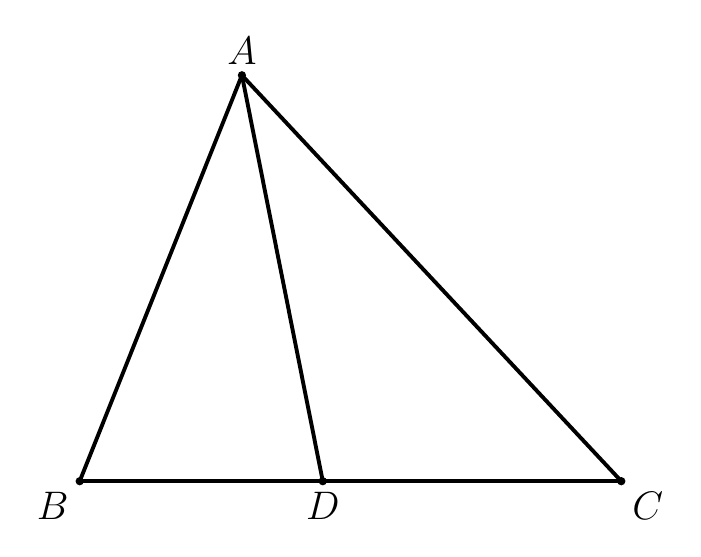
\begin{tikzpicture}[line join=round, line width=1.4pt]
  % Vertices (scale s = 0.018182 cm/px, centred on ink bbox)
  \coordinate (A) at (-1.438,2.573);
  \coordinate (B) at (-3.498,-2.582);
  \coordinate (C) at (3.380,-2.582);
  \coordinate (D) at (-0.411,-2.582);

  % Segments
  \draw (A) -- (B);
  \draw (A) -- (C);
  \draw (A) -- (D);
  \draw (B) -- (C);

  % Vertex dots
  \fill (A) circle (1.5pt);
  \fill (B) circle (1.5pt);
  \fill (C) circle (1.5pt);
  \fill (D) circle (1.5pt);

  % Labels
  \node[font=\fontsize{15}{18}\selectfont, above] at (A) {$A$};
  \node[font=\fontsize{15}{18}\selectfont, below left] at (B) {$B$};
  \node[font=\fontsize{15}{18}\selectfont, below right] at (C) {$C$};
  \node[font=\fontsize{15}{18}\selectfont, below] at (D) {$D$};
\end{tikzpicture}
\end{document}